\begin{figure}[t]
\centering
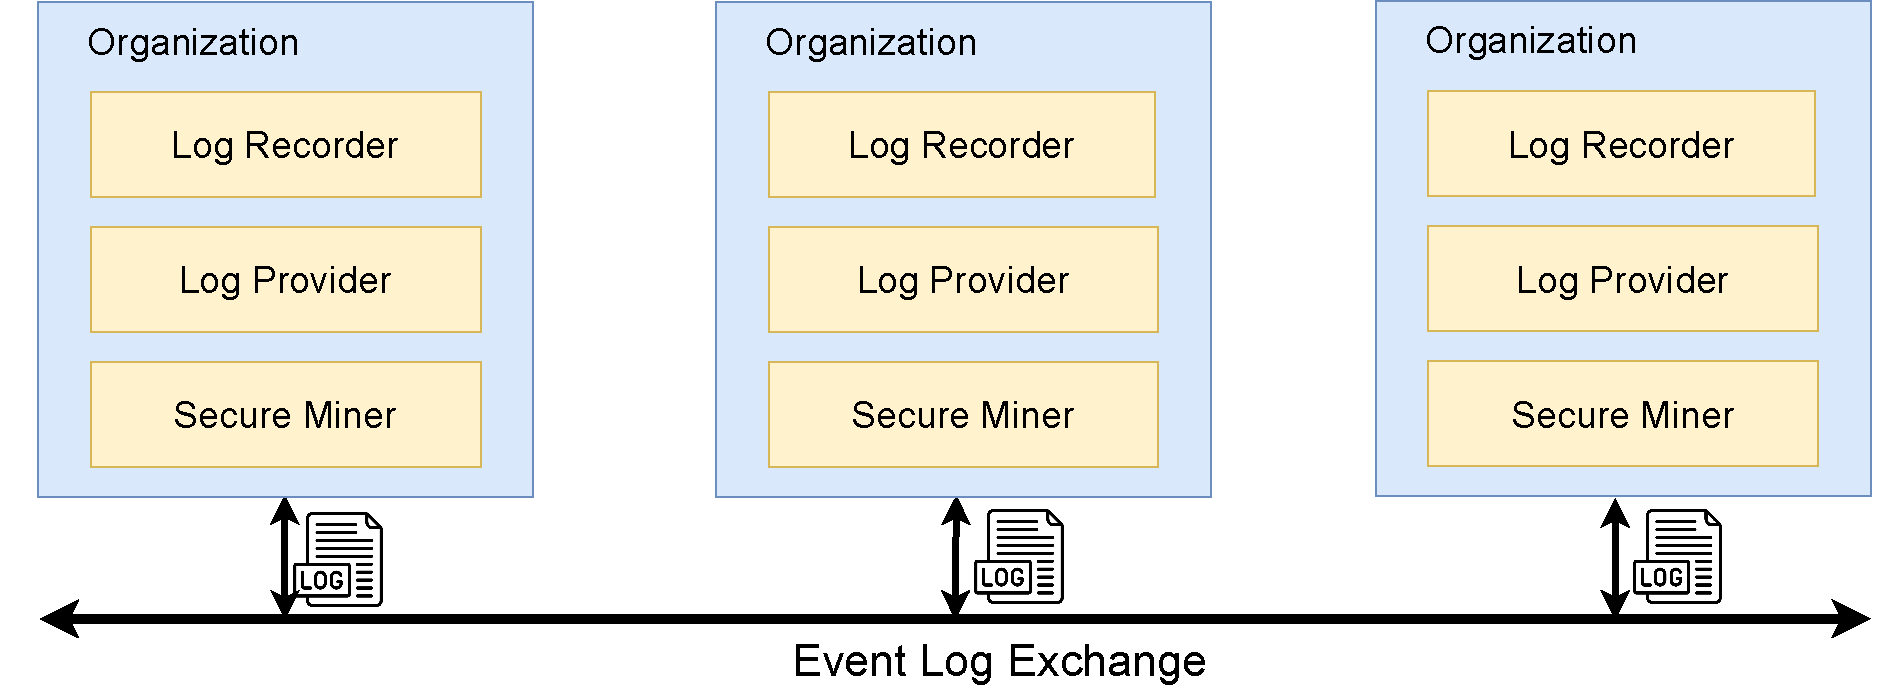
\includegraphics[width=11cm]{content/figures/architecture_diagram.pdf}
\caption{High-level architectural overview of the framework.}
\label{fig:architecture_diagram}
\end{figure}
In this section, we present the high-level architecture underlying our solution. We take into account each component individually. After that, we focus on the trusted miner component that represent the core of our contribution. Finally we provide an overview of the main interactions taking place between the introduced components.

\subsection{Architecture at large}
Our architecture involves networks of nodes controlled by different \texttt{Organization}s exchanging their event logs. \texttt{Organization}s in the same network collaborate to reach a common objective composing business processes whose event logs are scattered across multiple places. The hospital, the specialized clinic, and the pharmaceutic company mentioned in the running example, provide an example of partner \texttt{Organization}s. An \texttt{Organization} may assume one of the following two different roles or both: \textit{provider}, if it delivers event logs to be collaboratively mined; a \textit{miner} whenever it applies process mining algorithms using local event logs in combination with ones generated by providers. Each \texttt{Organization} is associated with an asymmetric public/private key pair through which it authenticates messages sent to other \texttt{Organizations}.

In \cref{fig:architecture_diagram}, we propose a high level schematization of our solution. Each \texttt{Organization} embeds four main components, which we describe next: the Process-Aware Information System (\texttt{PAIS}) and the \texttt{PAIS Interface}, the \texttt{Log Provider} and the \texttt{Trusted Miner}.


% \subsubsection{PAIS Interface.}
The \texttt{PAIS Interface} collects the logic to interact with the Process-aware Information Sytem (\texttt{PAIS}) of the \texttt{Organization}. \texttt{PAIS}s systems help \texttt{Organization}s to handle business processes including accounting and resource management. The maintenance of event logs is one of the core tasks performed by these systems~\cite{Dumas.etal/2018:FundamentalsofBPM}. In our architecture, we generalize the interaction with these systems through the \texttt{PAIS Interface}. The \texttt{PAIS Interface} is queried by the local \texttt{Log Provider} for event logs to be fed into \texttt{Trusted Miner}s. 


% \subsubsection{Log Provider.}
The \texttt{Log Provider} component delivers on-demand data to \texttt{Trusted Miner}s. % belonging to partner \texttt{Organization}s. 
It controls access to resources by verifying the identity of the miner %\texttt{Log Provider}s authenticate event log requests 
using asymetric encryption. %The goal of the authentication procedure is to extract the public key representing the identity of the sending \texttt{Trusted Miner}.

The \texttt{Trusted Miner} shelters external event logs inside an \texttt{Organization}'s system by preserving data confidentiality and integrity. We provide an in deepth focus on this component as follow.

\begin{figure}[t]
\centering
\includegraphics[width=7cm]{content/figures/trusted_miner.pdf}
\caption{Modules of the Trusted Miner component}
\label{fig:trusted_miner}
\end{figure}




\subsection{Trusted Miners in Reserved Zones}
%The \texttt{Trusted Miner} is a trusted application running inside the \texttt{Reserved Zone} that makes its source code and data tamper-proof. 
The main goal of the \texttt{Trusted Miner} is to allow \texttt{Organization}s to execute process mining algorithms using %local event logs alongside 
event logs retrieved from provider \texttt{Organization}s, offering fair data utilization to log providers. \texttt{Trusted Miners} are located in \texttt{Reserved Zone}s that guarantee tamperproofing and data confidentiality. In \cref{fig:trusted_miner}, we show an high level schematization of \texttt{Trusted Miner}s in which we distinguish four different modules: the \texttt{Trusted Memory}, the \texttt{Log Requester}, the \texttt{Log Receiver}, and the \texttt{Log Elaborator}.

Data contained in event logs belonging to provider \texttt{Organizaition}s are stored by miners in the \texttt{Trusted Memory}. This module relies on an hardware tecniques which makes event log manipuluations impossible from outside the \texttt{Reserved Zone}. Modules of the \texttt{Trusted Miner} are the only entities enabled to access data stored in the \texttt{Trusted Memory}. %Referring to our motivating scenario, the only way for the hospital to use the event logs retrieved from the specialized clinic is via the secure procedures offered by its \texttt{Trusted Miner}.

As we will see in \cref{sec:architecture:workflow}, the \texttt{Log Requester} and the \texttt{Log Receiver} are the fundamental modules that we employee during the event log exchange. \texttt{Log Requester}s initalize the exchange procedure and sends authenticable data requests to the \texttt{Data Provision} module of log providers. The \texttt{Log Receiver} collects event logs sent by \texttt{Log Providers} and store them in the \texttt{Trusted Memory}. This module offers methodologies that allow \texttt{Log Providers} to perform the remote attestation. Thanks to this  through wich it verifies that the \texttt{Log Requester} is actualy running in the \texttt{Reserved Zone}.% According to our running example, the hospital's \texttt{Log Receiver} must prove its trusted nature to the clinc and the pharmaceutical company's \texttt{Log Provider} before receiving event logs, showing that it is actually running in a \texttt{Reserved Zone}.

The \texttt{Log Elaborator} is the core module of the \texttt{Trusted Miner}. It collects the logic to execute process mining algorithms in the \texttt{Reserved Zone}. It support the integration of different family of tecniques such as \textit{process discovery}~\cite{citation}, \textit{conformance checking}~\cite{citation} and \textit{performance analysis}~\cite{ciation}. When activated, the \texttt{Log Elaborator} %interacts with the \texttt{Trusted Memory} in order to 
accesses external event logs stored inside the \texttt{Reserved Zone}. These are integrated with the local event log by the \texttt{Log Elaborator} via the merging procedure. During the merging, the \texttt{Log Elaborator} enriches local traces with events belonging to logs retrieved from partner \texttt{Organization}s.








\subsection{Workflow}
% \label{sec:architecture:workflow}
\subsubsection{Initialization}
\subsubsection{Data Exchange}
%The goal of the authentication procedure is to extract the public key representing the identity of the sending \texttt{Trusted Miner}.
%Remote Attestation and Log Segmentation are crucial procedures handled by the \texttt{Log Provider} during the provision process. Through Remote Attestation, \texttt{Log Provider}s verify that the \texttt{Trusted Miner} that has generated the log request  is: (i) a known software object running inside a Reserved Zone; (ii) controlled by a partner \texttt{Organization} that has rights to access the event log. We named Log Segementation the process through which \texttt{Log Provider}s split the event log to be delivered in sub-log of smaller size.
\subsubsection{Data Elaboration}



